\section{Simulation Analysis}
\label{sec:simulation}

In this section we will describe the simulation of the circuit \ref{fig:rc}.
The model for diodes chosen was the default model of \emph{Ngspice}.

Starting off, we used a smaller and simpler circuit that could achieve
the goal of the laboratory just to get a grasp of the circuit's behaviour.
Later we optimized the circuit with 3 objectives:
\begin{itemize}
  \item Reduce the cost of resistors, capacitors and diodes;
  \item Reduce the ripple of the signal;
  \item Get as close as posible to an average voltage of 12V.
\end{itemize}
Keeping that in mind, we immediately knew that using a full wave rectifer opposed to a half wave
was very much worth, given that the monetary cost of the diodes was low and the ripple impact using the full wave was massive.
The capacitance, resistance value and number of diodes were achieved by trial and error, trying to minimize the
ripple and $|V_{o}-12|$ given the total cost.

Moreover, the \emph{Ngspice}\textquotesingle s functions used to calculate the average value, maximum and minimum (these last two to calculate the ripple)
were respectively: AVG, MAX and MIN.

For the model of an ideal transformer, we used a current controlled current source on the side of the original input
and a voltage controlled voltage source on the other side.
The value of proportionality constant were the same in both and equal to n=1/15.
As to fulfill \emph{Ngspice}\textquotesingle s requirements for this setup to work we had to use a auxiliary voltage source with V=0
and a resistance with an absurd value (as to not pass current through it) to connect both circuits. We
emphasize that these last two would not exist in a real circuit and they are just a requirement for \emph{Ngspice} to work. The simulation results are
presented below.

\begin{figure}[h] \centering
  \includegraphics[scale=0.5]{spice_t3.pdf}
  \caption{Voltages at the output of the envelope detetctor (blue) and voltage regulator circuits (red).}
  \label{fig:11}
\end{figure}

\begin{figure}[h] \centering
  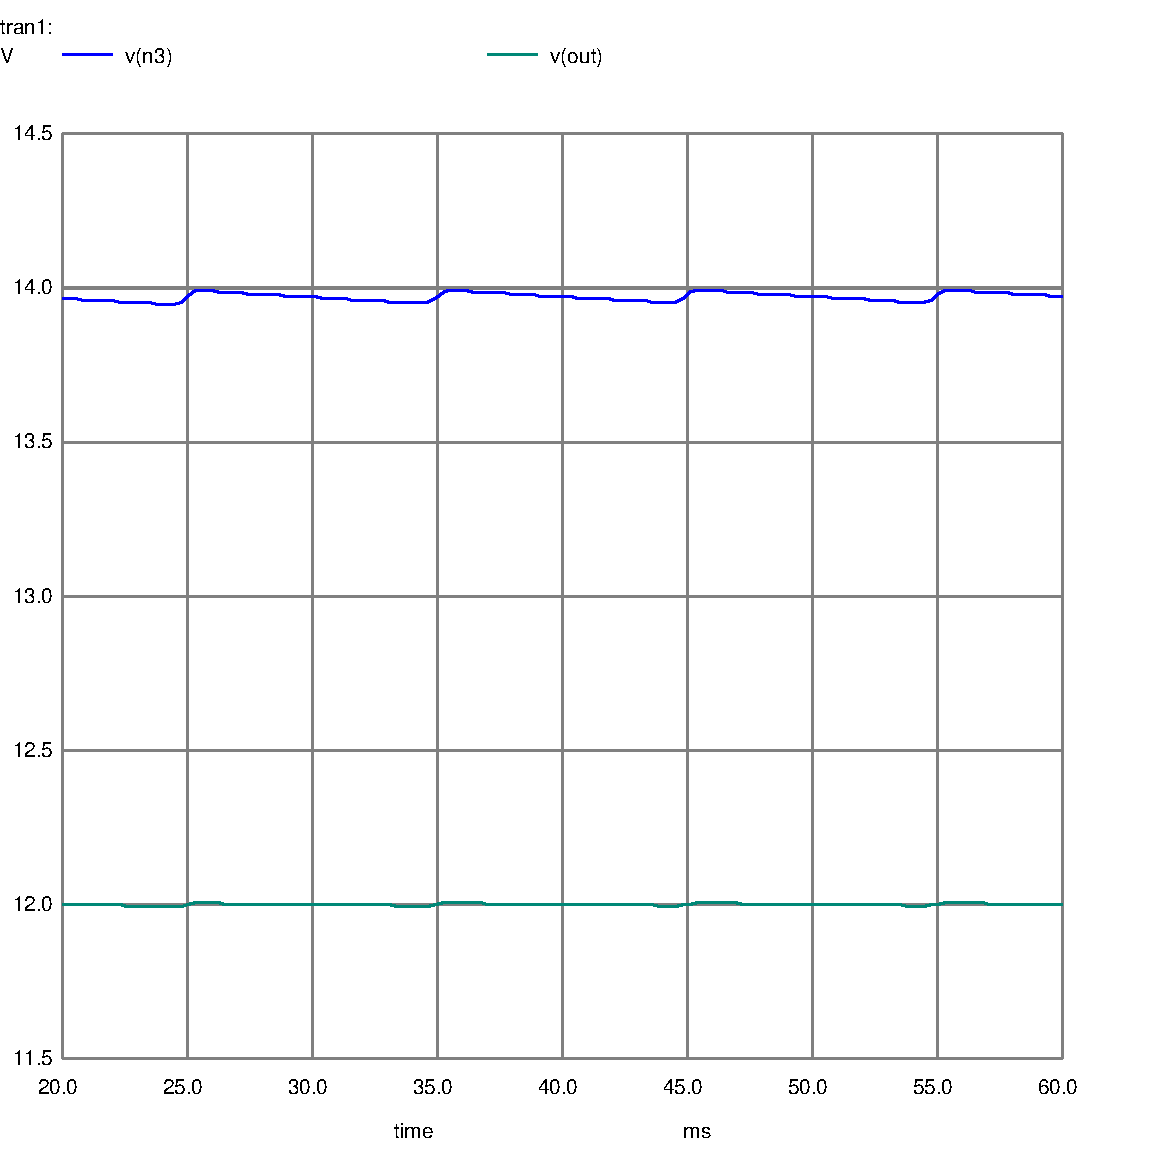
\includegraphics[scale=0.5]{Spice_t3_Zoom.pdf}
  \caption{Voltages at the output of the envelope detetctor (blue) and voltage regulator circuits (red): detail in the interval [20, 60] ms.}
  \label{fig:33}
\end{figure}

\begin{figure}[h] \centering
  \includegraphics[scale=0.5]{spice_t3_2.pdf}
  \caption{Output AC component (V(out)-12).}
  \label{fig:22}
\end{figure}

\clearpage

\begin{figure}[h] \centering
  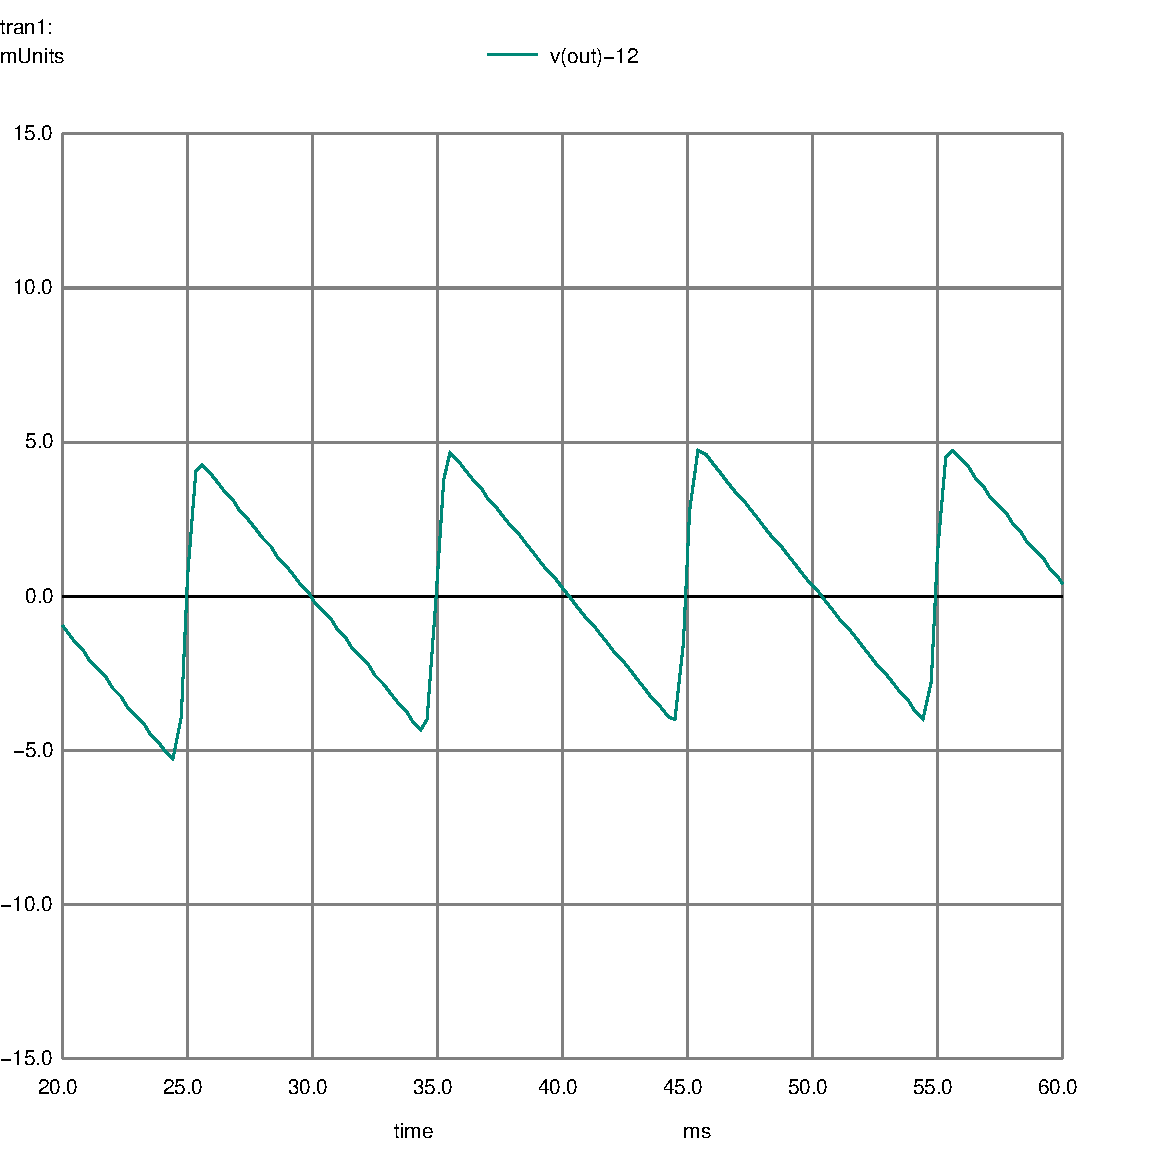
\includegraphics[scale=0.8]{Spice_t3_2_Zoom.pdf}
  \caption{Output AC component (V(out)-12): detail in the interval [20, 60] ms.}
  \label{fig:44}
\end{figure}

Overall, the results were highly satisfactory. The average output was very close to 12V ($\overline{V_{o}}=12.00002\hspace{1mm}V$)
and the ripple was really close to 0 ($Ripple=10.01000\hspace{1mm}mV$).
The total cost (in monetary units) was 44, leaving us with a merit of 2.265704, using the formula below:
\begin{equation}
  M=\dfrac{1}{cost\cdot \left( ripple\left( V_{0}\right) +\overline{\left( v_{0}-12\right) }+10^{-6}\right)} = 2.265704
\end{equation}
\begin{itemize}
  \item Resistors $\rightarrow$ 1 MU per k$\Omega$;
  \item Capacitors $\rightarrow$ 1 MU per $\mu$F;
  \item Diodes $\rightarrow$ 0.1 MU per diode.
\end{itemize}
